\begin{frame}{Համասեռ գրաֆների դեկարտյան արտադրյալներ}

(Գիառո, Կուբալ, 2004) Եթե $G,H\in \mathfrak{N}$, ապա 
\begin{center}
$w(G\square H)\leq w(G)+w(H)$
\end{center}
\begin{center}
$W(G\square H)\geq W(G)+W(H)$
\end{center}


\begin{theorem}[2.2.1]
Եթե $G,H\in \mathfrak{N}$, ընդ որում $H$-ը $r$-համասեռ է, ապա.
\begin{center}
$W(G\square H)\geq W(G)+W(H)+r$:
\end{center}
\end{theorem}
\end{frame}

\begin{frame}{Սեպարաբել միջակայքային ներկումներ}
\begin{columns}
\begin{column}{0.57\textwidth}
    Դիցուք $G$-ն կապակցված է:\\
    Ֆիքսված $x \in V(G)$ գագաթի համար՝\\
    \begin{center}
    $V(G) = \bigcup\limits_{i=0}^{\epsilon(x)}N_i(x)$, որտեղ
    \end{center}
    \begin{center}
    $N_i(x)=\left\{ v \in V(G) : d(v,x)=i \right\}$,
    \end{center}
    \begin{center}
    $i=0,\ldots,\epsilon(x)$: 
    \end{center}
\end{column}
\begin{column}{0.43\textwidth}
\begin{figure}[t]
\centering
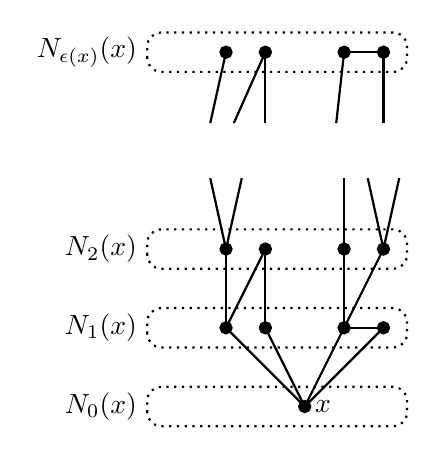
\begin{tikzpicture}[style=thick]
    \coordinate (V0) at (2cm,1cm);
    \coordinate (V11) at (1cm,2cm);
    \coordinate (V12) at (1.5cm,2cm);
    \coordinate (V13) at (2.5cm,2cm);
    \coordinate (V14) at (3cm,2cm);
    \coordinate (V21) at (1cm,3cm);
    \coordinate (V22) at (1.5cm,3cm);
    \coordinate (V23) at (2.5cm,3cm);
    \coordinate (V24) at (3cm,3cm);
    \coordinate (V31) at (0.8cm,3.9cm);
    \coordinate (V32) at (1.2cm,3.9cm);
    \coordinate (V33) at (2.5cm,3.9cm);
    \coordinate (V34) at (2.8cm,3.9cm);
    \coordinate (V35) at (3.2cm,3.9cm);
    \coordinate (V41) at (0.8cm,4.6cm);
    \coordinate (V42) at (1.1cm,4.6cm);
    \coordinate (V43) at (1.5cm,4.6cm);
    \coordinate (V44) at (2.4cm,4.6cm);
    \coordinate (V45) at (3cm,4.6cm);
    \coordinate (Vn1) at (1cm,5.5cm);
    \coordinate (Vn2) at (1.5cm,5.5cm);
    \coordinate (Vn3) at (2.5cm,5.5cm);
    \coordinate (Vn4) at (3cm,5.5cm);
    
    \draw (V0) -- (V11);
    \draw (V0) -- (V12);
    \draw (V0) -- (V13);
    \draw (V0) -- (V14);
    \draw (V13) -- (V14);
    
    \draw (V11) -- (V21);
    \draw (V11) -- (V22);
    \draw (V12) -- (V22);
    \draw (V13) -- (V23);
    \draw (V13) -- (V24);
    
    \draw (V21) -- (V31);
    \draw (V21) -- (V32);
    \draw (V23) -- (V33);
    \draw (V24) -- (V34);
    \draw (V24) -- (V35);
    
    \draw (V41) -- (Vn1);
    \draw (V42) -- (Vn2);
    \draw (V43) -- (Vn2);
    \draw (V44) -- (Vn3);
    \draw (V45) -- (Vn4);
    \draw (Vn3) -- (Vn4);
    
    \draw[dotted,rounded corners=5pt]
  (0,1) node[left]{$N_0(x)$} ++(0,-0.25) rectangle ++(3.3,0.5) ;
  
  \draw[dotted,rounded corners=5pt]
  (0,2) node[left]{$N_1(x)$} ++(0,-0.25) rectangle ++(3.3,0.5) ;
  
  \draw[dotted,rounded corners=5pt]
  (0,3) node[left]{$N_2(x)$} ++(0,-0.25) rectangle ++(3.3,0.5) ;
  \draw[dotted,rounded corners=5pt]
  (0,5.5) node[left]{$N_{\epsilon(x)}(x)$} ++(0,-0.25) rectangle ++(3.3,0.5) ;
    
    \draw[fill=black] (V0) circle (2pt) node[right]{$x$};
    \draw[fill=black] (V11) circle (2pt);
    \draw[fill=black] (V12) circle (2pt);
    \draw[fill=black] (V13) circle (2pt);
    \draw[fill=black] (V14) circle (2pt);
    \draw[fill=black] (V21) circle (2pt);
    \draw[fill=black] (V22) circle (2pt);
    \draw[fill=black] (V23) circle (2pt);
    \draw[fill=black] (V24) circle (2pt);
    \draw[fill=black] (Vn1) circle (2pt);
    \draw[fill=black] (Vn2) circle (2pt);
    \draw[fill=black] (Vn3) circle (2pt);
    \draw[fill=black] (Vn4) circle (2pt);
\end{tikzpicture}
\end{figure}
\end{column}
\end{columns}
\end{frame}

\begin{frame}{Սեպարաբել միջակայքային ներկումներ}
\begin{figure}[b!]
\centering
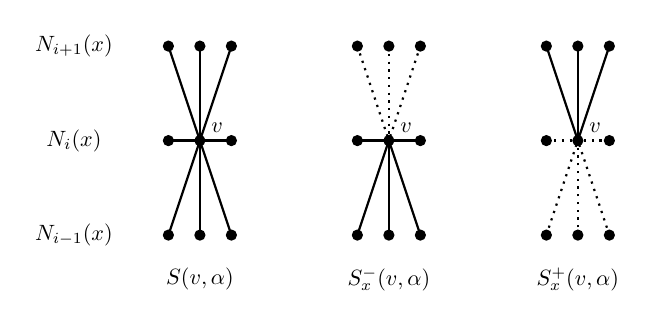
\begin{tikzpicture}[style=thick,scale=0.8, every node/.style={scale=0.8}]
    \node at (-0.5cm, 1cm) {$N_{i-1}(x)$};
    \node at (-0.5cm, 2.5cm) {$N_i(x)$};
    \node at (-0.5cm, 4cm) {$N_{i+1}(x)$};
    
% first sample
    \coordinate (V111) at (1cm,1cm);
    \coordinate (V112) at (1.5cm,1cm);
    \coordinate (V113) at (2cm,1cm);
    \coordinate (V121) at (1cm,2.5cm);
    \coordinate (V122) at (1.5cm,2.5cm);
    \coordinate (V123) at (2cm,2.5cm);
    \coordinate (V131) at (1cm,4cm);
    \coordinate (V132) at (1.5cm,4cm);
    \coordinate (V133) at (2cm,4cm);
    
    \draw (V111) -- (V122);
    \draw (V112) -- (V122);
    \draw (V113) -- (V122);
    \draw (V121) -- (V122);
    \draw (V123) -- (V122);
    \draw (V131) -- (V122);
    \draw (V132) -- (V122);
    \draw (V133) -- (V122);
    
    \draw[fill=black] (V111) circle (2pt);
    \draw[fill=black] (V112) circle (2pt);
    \draw[fill=black] (V113) circle (2pt);
    \draw[fill=black] (V121) circle (2pt);
    \draw[fill=black] (V122) circle (2pt) node[right] at (1.55cm,2.7cm) {$v$};
    \draw[fill=black] (V123) circle (2pt);
    \draw[fill=black] (V131) circle (2pt);
    \draw[fill=black] (V132) circle (2pt);
    \draw[fill=black] (V133) circle (2pt);
    
    \node at (1.5cm, 0.3cm) {$S(v,\alpha)$};
    
% second sample
    \coordinate (V211) at (4cm,1cm);
    \coordinate (V212) at (4.5cm,1cm);
    \coordinate (V213) at (5cm,1cm);
    \coordinate (V221) at (4cm,2.5cm);
    \coordinate (V222) at (4.5cm,2.5cm);
    \coordinate (V223) at (5cm,2.5cm);
    \coordinate (V231) at (4cm,4cm);
    \coordinate (V232) at (4.5cm,4cm);
    \coordinate (V233) at (5cm,4cm);
    
    \draw (V211) -- (V222);
    \draw (V212) -- (V222);
    \draw (V213) -- (V222);
    \draw (V221) -- (V222);
    \draw (V223) -- (V222);
    \draw[dotted] (V231) -- (V222);
    \draw[dotted] (V232) -- (V222);
    \draw[dotted] (V233) -- (V222);
    
    \draw[fill=black] (V211) circle (2pt);
    \draw[fill=black] (V212) circle (2pt);
    \draw[fill=black] (V213) circle (2pt);
    \draw[fill=black] (V221) circle (2pt);
    \draw[fill=black] (V222) circle (2pt) node[right] at (4.55cm,2.7cm) {$v$};
    \draw[fill=black] (V223) circle (2pt);
    \draw[fill=black] (V231) circle (2pt);
    \draw[fill=black] (V232) circle (2pt);
    \draw[fill=black] (V233) circle (2pt);
    
    \node at (4.5cm, 0.3cm) {$S_x^{-}(v,\alpha)$};
    
% third sample
    \coordinate (V311) at (7cm,1cm);
    \coordinate (V312) at (7.5cm,1cm);
    \coordinate (V313) at (8cm,1cm);
    \coordinate (V321) at (7cm,2.5cm);
    \coordinate (V322) at (7.5cm,2.5cm);
    \coordinate (V323) at (8cm,2.5cm);
    \coordinate (V331) at (7cm,4cm);
    \coordinate (V332) at (7.5cm,4cm);
    \coordinate (V333) at (8cm,4cm);
    
    \draw[dotted] (V311) -- (V322);
    \draw[dotted] (V312) -- (V322);
    \draw[dotted] (V313) -- (V322);
    \draw[dotted] (V321) -- (V322);
    \draw[dotted] (V323) -- (V322);
    \draw (V331) -- (V322);
    \draw (V332) -- (V322);
    \draw (V333) -- (V322);
    
    \draw[fill=black] (V311) circle (2pt);
    \draw[fill=black] (V312) circle (2pt);
    \draw[fill=black] (V313) circle (2pt);
    \draw[fill=black] (V321) circle (2pt);
    \draw[fill=black] (V322) circle (2pt) node[right] at (7.55cm,2.7cm) {$v$};
    \draw[fill=black] (V323) circle (2pt);
    \draw[fill=black] (V331) circle (2pt);
    \draw[fill=black] (V332) circle (2pt);
    \draw[fill=black] (V333) circle (2pt);
    
    \node at (7.5cm, 0.3cm) {$S_x^{+}(v,\alpha)$};
    
\end{tikzpicture}
\label{vertexSpectrums}
\end{figure}
\fontsize{10pt}{11}\selectfont

Բոլոր $v \in N_i(G)$ գագաթների սպեկտրները տրոհենք 2 մասի.
\begin{align*}
S_x^-(v,\alpha) &= \left\{ \alpha(vu) : u\in N_{i-1}(x) \cup N_i(x) \right\}\\
S_x^+(v,\alpha) &= \left\{ \alpha(vu) : u\in N_{i+1}(x) \right\}
\end{align*}

Կասենք, որ $G$ կապակցված գրաֆի $\alpha$ միջակայքային ներկումը \textbf{սեպարաբել} է $x$ գագաթի նկատմամբ, եթե ցանկացած $\forall v \in V(G)$ գագաթի համար $\max S_x^-(v,\alpha) < \min S_x^+(v,\alpha)$:
\end{frame}

\begin{frame}{Սեպարաբել միջակայքային ներկումներ}
\begin{columns}
\begin{column}{0.5\textwidth}
   \begin{theorem}[2.2.4]
    Դիցուք $G$ կապակցված գրաֆը ունի սեպարաբել միջակայքային $t_G$-ներկում որևէ $x\in V(G)$ գագաթի նկատմամբ, ընդ որում գոյություն ունի $y\in N_{\epsilon(x)}(x)$ գագաթ, որի սպեկտրը պարունակում է $t_G$ գույնը, իսկ $1\in S(x,\alpha)$: Եթե $H$ գրաֆը $r$-համասեռ է և ունի միջակայքային $t_H$-ներկում, ապա
    \begin{center}
    $W(G \square H) \geq t_G + t_H + \epsilon(x)r$:
    \end{center}
    \end{theorem}

\end{column}
\begin{column}{0.5\textwidth}  %%<--- here
    \begin{figure}[t]
\centering
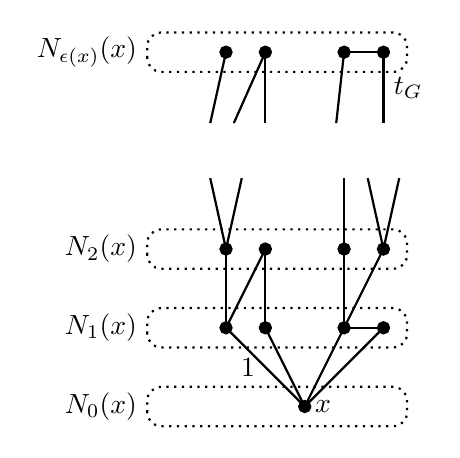
\begin{tikzpicture}[style=thick]
    \coordinate (V0) at (2cm,1cm);
    \coordinate (V11) at (1cm,2cm);
    \coordinate (V12) at (1.5cm,2cm);
    \coordinate (V13) at (2.5cm,2cm);
    \coordinate (V14) at (3cm,2cm);
    \coordinate (V21) at (1cm,3cm);
    \coordinate (V22) at (1.5cm,3cm);
    \coordinate (V23) at (2.5cm,3cm);
    \coordinate (V24) at (3cm,3cm);
    \coordinate (V31) at (0.8cm,3.9cm);
    \coordinate (V32) at (1.2cm,3.9cm);
    \coordinate (V33) at (2.5cm,3.9cm);
    \coordinate (V34) at (2.8cm,3.9cm);
    \coordinate (V35) at (3.2cm,3.9cm);
    \coordinate (V41) at (0.8cm,4.6cm);
    \coordinate (V42) at (1.1cm,4.6cm);
    \coordinate (V43) at (1.5cm,4.6cm);
    \coordinate (V44) at (2.4cm,4.6cm);
    \coordinate (V45) at (3cm,4.6cm);
    \coordinate (Vn1) at (1cm,5.5cm);
    \coordinate (Vn2) at (1.5cm,5.5cm);
    \coordinate (Vn3) at (2.5cm,5.5cm);
    \coordinate (Vn4) at (3cm,5.5cm);
    
    \draw (V0) -- node[left] {$1$} (V11);
    \draw (V0) -- (V12);
    \draw (V0) -- (V13);
    \draw (V0) -- (V14);
    \draw (V13) -- (V14);
    
    \draw (V11) -- (V21);
    \draw (V11) -- (V22);
    \draw (V12) -- (V22);
    \draw (V13) -- (V23);
    \draw (V13) -- (V24);
    
    \draw (V21) -- (V31);
    \draw (V21) -- (V32);
    \draw (V23) -- (V33);
    \draw (V24) -- (V34);
    \draw (V24) -- (V35);
    
    \draw (V41) -- (Vn1);
    \draw (V42) -- (Vn2);
    \draw (V43) -- (Vn2);
    \draw (V44) -- (Vn3);
    \draw (V45) -- node[right] {$t_G$} (Vn4);
    \draw (Vn3) -- (Vn4);
    
    \draw[dotted,rounded corners=5pt]
  (0,1) node[left]{$N_0(x)$} ++(0,-0.25) rectangle ++(3.3,0.5) ;
  
  \draw[dotted,rounded corners=5pt]
  (0,2) node[left]{$N_1(x)$} ++(0,-0.25) rectangle ++(3.3,0.5) ;
  
  \draw[dotted,rounded corners=5pt]
  (0,3) node[left]{$N_2(x)$} ++(0,-0.25) rectangle ++(3.3,0.5) ;
  \draw[dotted,rounded corners=5pt]
  (0,5.5) node[left]{$N_{\epsilon(x)}(x)$} ++(0,-0.25) rectangle ++(3.3,0.5) ;
    
    \draw[fill=black] (V0) circle (2pt) node[right]{$x$};
    \draw[fill=black] (V11) circle (2pt);
    \draw[fill=black] (V12) circle (2pt);
    \draw[fill=black] (V13) circle (2pt);
    \draw[fill=black] (V14) circle (2pt);
    \draw[fill=black] (V21) circle (2pt);
    \draw[fill=black] (V22) circle (2pt);
    \draw[fill=black] (V23) circle (2pt);
    \draw[fill=black] (V24) circle (2pt);
    \draw[fill=black] (Vn1) circle (2pt);
    \draw[fill=black] (Vn2) circle (2pt);
    \draw[fill=black] (Vn3) circle (2pt);
    \draw[fill=black] (Vn4) circle (2pt);
\end{tikzpicture}
\end{figure}

\end{column}
\end{columns}
\end{frame}

\begin{frame}{Սեպարաբել միջակայքային ներկումներ}

\begin{figure}[t!]
\centering
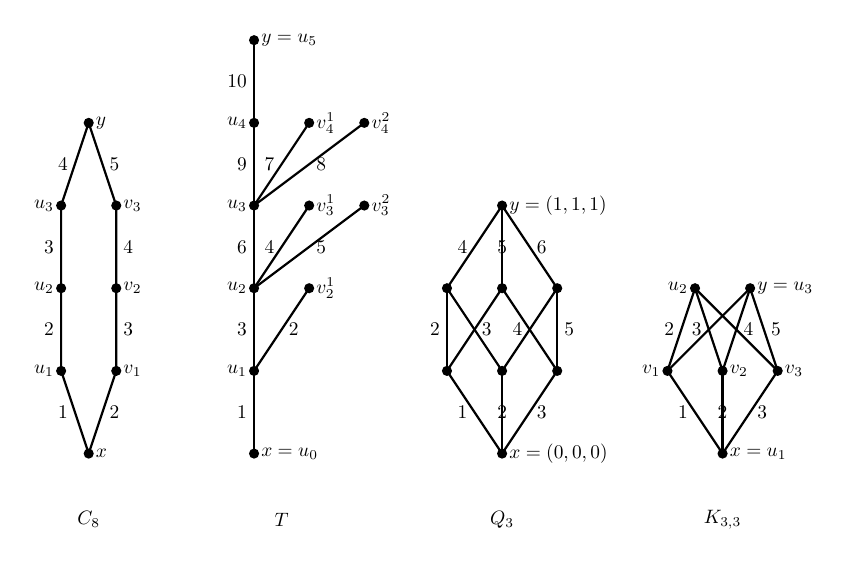
\begin{tikzpicture}[style=thick,scale=0.7, every node/.style={scale=0.7}]
% C_8
    \coordinate (c0) at (-0.5cm,1.5cm);
    \coordinate (c11) at (-1cm,3cm);
    \coordinate (c12) at (-1cm,4.5cm);
    \coordinate (c13) at (-1cm,6cm);
    \coordinate (c21) at (0cm,3cm);
    \coordinate (c22) at (0cm,4.5cm);
    \coordinate (c23) at (0cm,6cm);
    \coordinate (c4) at (-0.5cm,7.5cm);
    
    \draw (c0) -- node[left] {$1$} (c11) 
    -- node[left] {$2$} (c12) 
    -- node[left] {$3$} (c13) 
    -- node[left] {$4$} (c4);
    \draw (c0) -- node[right] {$2$} (c21) 
    -- node[right] {$3$} (c22) 
    -- node[right] {$4$} (c23) 
    -- node[right] {$5$} (c4);
    
    \draw[fill=black] (c0) circle (2pt)  node[right] {$x$};
    \draw[fill=black] (c11) circle (2pt) node[left] {$u_1$};
    \draw[fill=black] (c12) circle (2pt) node[left] {$u_2$};
    \draw[fill=black] (c13) circle (2pt) node[left] {$u_3$};
    \draw[fill=black] (c21) circle (2pt) node[right] {$v_1$};
    \draw[fill=black] (c22) circle (2pt) node[right] {$v_2$};
    \draw[fill=black] (c23) circle (2pt) node[right] {$v_3$};
    \draw[fill=black] (c4) circle (2pt) node[right] {$y$};
    
    \node at (-0.5cm, 0.3cm) {$C_8$};
    
% Caterpillar
    \coordinate (t0) at (2.5cm,1.5cm);
    \coordinate (t1) at (2.5cm,3cm);
    \coordinate (t21) at (2.5cm,4.5cm);
    \coordinate (t22) at (3.5cm,4.5cm);
    
    \coordinate (t31) at (2.5cm,6cm);
    \coordinate (t32) at (3.5cm,6cm);
    \coordinate (t33) at (4.5cm,6cm);
    
    \coordinate (t41) at (2.5cm,7.5cm);
    \coordinate (t42) at (3.5cm,7.5cm);
    \coordinate (t43) at (4.5cm,7.5cm);
    
    \coordinate (t5) at (2.5cm,9cm);
    
    \draw (t0) -- node[left] {$1$} (t1);
    \draw (t1) -- node[left] {$3$} (t21);
    \draw (t1) -- node[right] {$2$} (t22);
    \draw (t21) -- node[left] {$6$} (t31);
    \draw (t21) -- node[left] {$4$} (t32);
    \draw (t21) -- node[right] {$5$} (t33);
    \draw (t31) -- node[left] {$9$} (t41);
    \draw (t31) -- node[left] {$7$} (t42);
    \draw (t31) -- node[right] {$8$} (t43);
    \draw (t41) -- node[left] {$10$} (t5);
    
    \draw[fill=black] (t0) circle (2pt)  node[right] {$x=u_0$};
    \draw[fill=black] (t1) circle (2pt) node[left] {$u_1$};
    \draw[fill=black] (t21) circle (2pt) node[left] {$u_2$};
    \draw[fill=black] (t22) circle (2pt) node[right] {$v_2^1$};
    \draw[fill=black] (t31) circle (2pt) node[left] {$u_3$};
    \draw[fill=black] (t32) circle (2pt) node[right] {$v_3^1$};
    \draw[fill=black] (t33) circle (2pt) node[right] {$v_3^2$};
    \draw[fill=black] (t41) circle (2pt) node[left] {$u_4$};
    \draw[fill=black] (t42) circle (2pt) node[right] {$v_4^1$};
    \draw[fill=black] (t43) circle (2pt) node[right] {$v_4^2$};
    \draw[fill=black] (t5) circle (2pt)  node[right] {$y=u_5$};
    
    \node at (3cm, 0.3cm) {$T$};
    
    
% Q_3
    \coordinate (q000) at (7cm,1.5cm);
    \coordinate (q100) at (6cm,3cm);
    \coordinate (q010) at (7cm,3cm);
    \coordinate (q001) at (8cm,3cm);
    
    \coordinate (q110) at (6cm,4.5cm);
    \coordinate (q101) at (7cm,4.5cm);
    \coordinate (q011) at (8cm,4.5cm);
    \coordinate (q111) at (7cm,6cm);
    
    \draw (q000) -- node[left] {$1$} (q100);
    \draw (q000) -- node {$2$} (q010);
    \draw (q000) -- node[right] {$3$} (q001);
    
    \draw (q100) -- node[left] {$2$} (q110);
    \draw (q100) --  (q101);
    \draw (q010) -- node[right] {$3$} (q110);
    \draw (q010) --  (q011);
    \draw (q001) -- node[left] {$4$} (q101);
    \draw (q001) -- node[right] {$5$} (q011);
    
    \draw (q110) -- node[left] {$4$} (q111);
    \draw (q101) -- node {$5$} (q111);
    \draw (q011) -- node[right] {$6$} (q111);
    
    \draw[fill=black] (q000) circle (2pt)  node[right] {$x=(0,0,0)$};
    \draw[fill=black] (q100) circle (2pt);  
    \draw[fill=black] (q010) circle (2pt);  
    \draw[fill=black] (q001) circle (2pt);  
    \draw[fill=black] (q110) circle (2pt);  
    \draw[fill=black] (q101) circle (2pt);  
    \draw[fill=black] (q011) circle (2pt);  
    \draw[fill=black] (q111) circle (2pt) node[right] {$y=(1,1,1)$};  
    
    \node at (7cm, 0.3cm) {$Q_3$};
    
    
% K_3,3
    \coordinate (b0) at (11cm,1.5cm);
    \coordinate (b11) at (10cm,3cm);
    \coordinate (b12) at (11cm,3cm);
    \coordinate (b13) at (12cm,3cm);
    
    \coordinate (b21) at (10.5cm,4.5cm);
    \coordinate (b22) at (11.5cm,4.5cm);
    
    \draw (b0) -- node[left] {$1$} (b11);
    \draw (b0) -- node {$2$} (b12);
    \draw (b0) -- node[right] {$3$} (b13);
    
    \draw (b11) -- node[left] {$2$} (b21);
    \draw (b11) -- node[left] {$3$} (b22);
    \draw (b12) --  (b21);
    \draw (b12) --  (b22);
    \draw (b13) -- node[right] {$4$} (b21);
    \draw (b13) -- node[right] {$5$} (b22);
    
    \draw[fill=black] (b0) circle (2pt)  node[right] {$x=u_1$};
    \draw[fill=black] (b11) circle (2pt)  node[left] {$v_1$};  
    \draw[fill=black] (b12) circle (2pt)  node[right] {$v_2$};  
    \draw[fill=black] (b13) circle (2pt)  node[right] {$v_3$};  
    \draw[fill=black] (b21) circle (2pt)  node[left] {$u_2$};  
    \draw[fill=black] (b22) circle (2pt)  node[right] {$y=u_3$};  
    
    \node at (11cm, 0.3cm) {$K_{3,3}$};
    
    
\end{tikzpicture}
\end{figure}
\end{frame}

\begin{frame}[shrink]{Սեպարաբել միջակայքային ներկումներ}

\begin{corollary}[2.2.5]
Եթե $G$-ն հանդիսանում է 
\begin{itemize}
\item զույգ երկարությամբ ցիկլ,
\item շղթա,
\item n-չափանի խորանարդ,
\item թրթուրածառ կամ
\item լրիվ երկկողմանի գրաֆ,
\end{itemize}
իսկ $H$-ը միջակայքային ներկելի $r$-համասեռ գրաֆ է, ապա
\begin{center}
$W(G \square H) \geq W(G) + W(H) + \mathrm{diam}(G)r$:
\end{center}
\end{corollary}

\end{frame}